
\section{Word Embeddings}


\begin{frame}{Word Embeddings: Definition}




    \begin{itemizeSpaced}{7pt}
        \item \textbf{Word embeddings} or \textbf{latent vector representations} are fixed-length vector representations of words. 
        
        \item Have led to the success of many NLP systems in recent years, across tasks like named entity recognition (NER), semantic parsing (SP), part of speech tagging (POS), and semantic role labeling (SRL) (Luong et al. 2013, p. 1).
        
    \end{itemizeSpaced}
    
    Example word vectors are in \cref{fig:exampleWordEmb}
    
    \begin{figure}[h]
    %\vspace{-10pt}
    \centering
    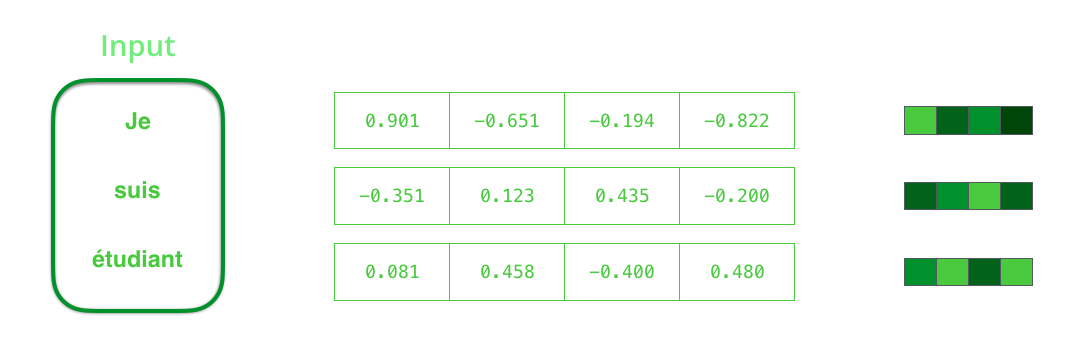
\includegraphics[width=0.8\textwidth]{imgs/example_word_embedding.png}
    %\vspace{-10pt}
    \caption{\scriptsize Example Word Embeddings. From \emph{Visualizing Neural Machine Translation Mechanics of Seq2Seq Models with Attention}, by Jay Alammar, 2018. \url{http://jalammar.github.io/visualizing-neural-machine-translation-mechanics-of-seq2seq-models-with-attention/}. Copyright 2018 by Jay Alammar.}
    %\vspace{-10pt}
    \label{fig:exampleWordEmb}
    \end{figure}
    
\end{frame}



\begin{frame}{Word Embedding: Definition}
    
    \begin{itemizeSpaced}{4pt}
        \item Word embeddings are unsupervised models that capture semantic and syntactic information about words in a compact low-dimensional vector representation. 
        
        \begin{itemizeSpaced}{0pt}
            \item \textbf{Example 1: } GloVe and Word2Vec are count models.
        
            \item \textbf{Example 2: }ERNIE 2.0 goes beyond simple co-occurrences (recognizes there is conceptual information tucked away in entities and phrases).
        \end{itemizeSpaced}
        
        \item Generally, these learned vector representations are then useful for reasoning about word usage and meaning (Melamud et al. 2016, p. 1).
        
        \item Different kinds: embeddings can be tokenized from sentences, phrases, characters, or just individual words. 
        \begin{itemizeSpaced}{2pt}
            \item Character embeddings are good at modeling \emph{morphology}
        \end{itemizeSpaced}
        
        \item Can capture \textbf{vector space semantics}. Famous word analogy ``man is to woman as king is to queen" is expressed using arithmetic on learned word vectors: $vector(man) - vector(woman) = vector(king) - vector(queen)$ (Smith, 2019).
        
        \item \textbf{Mathematically, How Models Make Embeddings: }
        \begin{itemizeSpaced}{0pt}
            \item a word’s conditional probability combines its \emph{embedding} and \emph{context vectors} of surrounding words, with different methods combining them differently. 
            
            \item Then, embeddings are fitted to text by maximizing the conditional probabilities of observed text (Rudolph et al. 2017).
        \end{itemizeSpaced}
    \end{itemizeSpaced}
    
    
\end{frame}





\begin{frame}{Word Embeddings: Usage}

\textbf{Key Ideas in NLP:} 

\begin{itemizeSpaced}{7pt}
    \item words used in similar ways have similar meanings (Firth, 1957). (Words in the same neighboring context may have similar meaning). 
    
    \begin{itemizeSpaced}{0pt}
        \item \textbf{distributed representations}\footnotemark of words in a vector space help models learn at  nlp tasks by grouping similar words (Mikolov et al. 2013a, p. 1).

    \end{itemizeSpaced}
    
    \item concepts in text corpora can be mined by machines.
    
    \item \textbf{Power of Word Embeddings:} can generalize to a class of similar sentences

    \begin{itemizeSpaced}{0pt}
        \item ``the wall is blue” to ``the ceiling is red” (Smith, 2019, p. 4).
    \end{itemizeSpaced}    

    
\end{itemizeSpaced}

\footnotetext[1]{\textbf{Distributed representation} of a word means information of that word is distributed across vector dimensions (Lenci, 2018). N-gram model is considered a \textbf{local representation} because it uses short context.}

\end{frame}





\begin{frame}{What is Polysemy?}
    %\large 
    
    \begin{definitionBlock}{Definition}
    \alert{\textbf{Polysemy}} means a word has multiple senses. 
    \end{definitionBlock}
    
    
    \begin{definitionBlock}{Definition}
    \alert{\textbf{Distributional hypothesis}} in NLP says meaning depends on context, and words in same contexts have similar meaning (Wiedemann et al., 2019). 
    \end{definitionBlock}
\end{frame}


\begin{frame}{Static vs. Contextual Embeddings}

\begin{itemizeSpaced}{5pt}
    \item Classic word vectors are called \textbf{static embeddings}. They represent each word with a single vector, regardless of its context (Ethayarajh, 2019). 
    
    
    % Filling block bg colors
    \metroset{block=fill}
    
    \begin{exampleBlock}{Example}
        Skip-Gram and Glove produce these ``context-free" representations because they use co-occurrence counts, not the more dynamic \textbf{language modeling} approach (Batista, 2018). 
    \end{exampleBlock}
    
    \begin{alertBlock}{Alert}
        All senses of a polysemic word are \emph{collapsed} within a single vector representation (Ethayarajh, 2019). 
        
        This can confuse models.
        
        ``Plant”'s embedding would be the ``average of its different contextual semantics relating to biology, placement, manufacturing, and power generation” (Neelakantan et al., 2015).

    
    \end{alertBlock}
      
\end{itemizeSpaced}
    
\end{frame}




\begin{frame}{Better: Contextual Embeddings (CWE)}

%{\large 
\begin{definitionBlock}{Definition}
    A \alert{contextual word embedding (CWE)} captures context using forward and backward history, using a bidirectional language model (biLM) (Antonio, 2019). 
    
    Static word embeddings are like ``look-up tables" but contextual embeddings have word type information (Smith, 2019). 
\end{definitionBlock}
%}

\begin{itemizeSpaced}{7pt}

    \item Abandoning the idea of using a fixed word sense inventory (to model polysemy) allows CWE's to create create a vector representation for each \textbf{word type} in the vocabulary and each \textbf{word token} in a context. 
    
    \item Experimentally, contextual are superior to static embeddings.
    
    \item ``sentence or context-level semantics together with word-level semantics proved to be a powerful innovation” in the NLP world (Wiedemann et al., 2019).
    
    
\end{itemizeSpaced}
    
\end{frame}